\subsection{连通空间与连通集}

定义 1. 如果拓扑空间 X 不是两个不相交的非空开集的并，就称它是连通的。

把“开集”一词换成“闭集”，便得到一个等价的定义。X 连通当且仅当 X 中既开又闭的子集只有空集与全空间 X 两者。

若 X 连通，且 A, B 是两个非空的开（相应地，闭）子集，使得 \(A \cup B = X\)，则 \(A \cap B \neq \varnothing\)。

例. * 1) 我们将在第四章，§ 2，第 5 目看到，实直线是连通的，而有理直线不是连通的。*

\begin{enumerate}
\def\labelenumi{\arabic{enumi})}
\setcounter{enumi}{1}
\tightlist
\item
  多于一个点的离散空间不是连通的。
\end{enumerate}

注意，若 \((\mathbf{U}_{t})_{t\in\mathbf{I}}\) 是由开集组成的拓扑空间 X 的一个分拆{[}由分拆的定义（见《集合论》，R，§ 4，第 4 目），这些开集必然非空{]}，则每个 \(U_{t}\) 在 X 中既开又闭，因为 \(U_{t}\) 的余集是诸 \(U_{x}\)（其中 \(x\neq t\)）的并。X 的开子集正是这样的子集 A：\(A\cap U_{t}\) 在 \(U_{t}\) 中是开的（对每个 \(t\in I\)），因而 X 可等同于诸 \(U_{t}\) 的和（§ 2，第 4 目，例 3），且当 I 多于一个元素时 X 不连通。

定义 2. 如果拓扑空间 X 的子集 A 作为 X 的子空间是连通的，就称 A 为一个连通集。

A 是 X 的连通子集的必要充分条件是：对 A 的每个由 X 的两个开（或闭）子集 B, C 组成的覆盖，只要 \(A \cap B\) 与 \(A \cap C\) 都非空，就有 \(A \cap B \cap C \neq \emptyset\)。

例. 在任何拓扑空间中，空集与每个由单独一点组成的集合都是连通的。在豪斯多夫空间 X 中，多于一个点的有限集都不连通；更一般地，X 中每个多于一个点且至少有一个孤立点的子集都不连通。

若稠密子集 A 连通，则全空间 X 连通；否则将存在 X 的两个非空不相交的开子集 M, N，使得 \(M \cup N = X\)，而 \(M \cap A\), \(N \cap A\) 将是 A 的两个不相交的非空开子集，其并为 A。于是我们有

命题 1. 若 A 是连通集，则每个满足 \(A \subset B \subset \overline{A}\) 的集合 B 都是连通的。

命题 2. 交非空的连通集族之并是连通的。

设 \((\mathbf{A}_t)_{i\in I}\) 是 \(\mathbf{X}\) 的连通子集的一个族，它们都含有同一个点 \(x\)；我们须证明

\[
\mathbf {A} = \bigcup_ {i} \mathbf {A} _ {i}
\]

是连通的。若不然，存在两个开集 B 与 C，使得 \(B \cap A\) 与 \(C \cap A\) 非空，且 \(A \subset B \cup C\) 及 \(A \cap B \cap C = \varnothing\)。x 属于 B, C 两集之一，设 \(x \in B\)；另一方面，诸集合 \(A_t\) 之一，设为 \(A_x\)，与 C 相交；因此我们有 \(A_x \subset B \cup C\)，\(A_x \cap B \cap C = \varnothing\)，且 \(B \cap A_x\) 与 \(C \cap A_x\) 非空。于是 \(A_x\) 不连通，这就得出矛盾。

推论. 设 \((\mathbf{A}_n)_{n\geqslant 0}\) 是连通集的一个无穷序列，使得 \(\mathbf{A}_{n + 1}\cap \mathbf{A}_n\neq \emptyset\) 对每个 \(n\geqslant 0\) 成立。则并 \(\bigcup_{n = 0}^{\infty}\mathbf{A}_n\) 是连通的。

对 \(n\) 用归纳法，由命题 2 立即看出，集合 \(\mathbf{B}_n = \bigcup_{i=0}^n \mathbf{A}_i\) 对每个 \(n\) 都是连通的。诸集合 \(\mathbf{B}_n\) 的交非空；故其并（等于 \(\bigcup_{n=0}^{\infty} \mathbf{A}_n\)）由命题 2 是连通的。

命题 3. 设 A 是拓扑空间 X 的一个子集。若 B 是 X 的连通子集，且同时与 A 和 \(\mathbb{C}\) A 相交，则 B 与 A 的边界相交。

若不然，B 与 A 的内部及外部的交将是 B 的两个开子集，且构成 B 的一个分拆，从而 B 将不连通。

推论. 在连通空间 X 中，每个异于 X 自身的非空集都至少有一个边界点。

\subsection{连通集在连续映射下的像}

命题 4. 设 A 是拓扑空间 X 的连通子集，f 是 X 到拓扑空间 X' 中的一个连续映射。则 \(f(\mathbf{A})\) 是连通的。

设 \(f(\mathbf{A})\) 不连通。则存在两个集合 \(\mathbf{M}'\), \(\mathbf{N}'\)，它们在 \(f(\mathbf{A})\) 中是开的，且构成 \(f(\mathbf{A})\) 的一个分拆；于是 \(\mathbf{A} \cap \overline{f}^{1}(\mathbf{M}')\) 与 \(\mathbf{A} \cap \overline{f}^{1}(\mathbf{N}')\) 在 \(\mathbf{A}\) 中是开的，且构成 \(\mathbf{A}\) 的一个分拆；这与 \(\mathbf{A}\) 连通的假设相矛盾。

连通集在连续映射下的逆像未必连通；例如考虑一个离散空间到一个由单独一点组成的空间中的映射。

由命题 4 我们得到不连通空间的另一个刻画：

命题 5. 拓扑空间 X 不连通的必要充分条件是：存在一个 X 到含有多于一个点的离散空间上的连续满射。

由命题 4，该条件是充分的。反之，若 X 不连通，则存在两个非空不相交的开子集 A, B，其并为 X，而 X 到两个元素的离散空间 \(\{a, b\}\) 上的映射 f（由 \(f(A) = \{a\}\) 与 \(f(B) = \{b\}\) 定义）是连续的。

\subsection{连通空间的商空间}

命题 6. 连通空间的每个商空间都是连通的。

这是第 2 目命题 4 的直接推论。

命题 7. 设 X 是一个拓扑空间，R 是 X 上的一个等价关系。若商空间 X/R 连通，且每个模 R 的等价类都连通，则 X 连通。

设 X 不连通。则存在 X 的一个分成两个开集 A, B 的分拆。集合 A, B 关于 R 是饱和的；因为若 \(x \in A\)，则 x 的等价类 M 不能与 B 相交，否则集合 \(A \cap M\), \(B \cap M\) 将构成 M 的一个分成两个在 M 中为开的集合的分拆，而这不可能，因为 M 是连通的。于是 A 与 B 的典范像是 X/R 中的开集，且构成 X/R 的一个分拆；这与 X/R 连通的假设相矛盾。

\subsection{连通空间的积}

命题 8. 连通空间的每个积都是连通的。反之，若非空空间的一个积连通，则每个因子都连通。

设 \(\mathbf{X} = \prod_{i \in I} \mathbf{X}_i\) 是拓扑空间的一个积。若诸 \(\mathbf{X}_i\) 非空，则有 \(\mathbf{X}_i = \text{pr}_i\mathbf{X}\)（对每个 \(i \in I\)）；因而若 \(\mathbf{X}\) 连通，则诸 \(\mathbf{X}_i\) 也连通（第 2 目，命题 4）。反之，设诸 \(\mathbf{X}_i\) 都连通而 \(\mathbf{X}\) 不连通。由第 2 目命题 5，存在一个连续满射 \(f: \mathbf{X} \to \mathbf{X}'\)，其中 \(\mathbf{X}'\) 是含有多于一个点的离散空间。设 \(a = (a_i)\) 是 \(\mathbf{X}\) 的任意一点，\(x\) 是任意指标；部分映射 \(f_x: \mathbf{X}_x \to \mathbf{X}'\) 由 \(f_x(x) = f((y_i))\) 定义，其中 \(y_x = x\)，而 \(y_i = a_i\)（若 \(i \neq x\)），它在 \(\mathbf{X}_x\) 上是连续的；由于 \(\mathbf{X}_x\) 连通，\(f_x\) 必在 \(\mathbf{X}_x\) 上取常值。由归纳法立即得出，\(f(x) = f(a)\) 对一切点 \(x = (x_i)\)（其中 \(x_i = a_i\) 除有限多个指标 \(i \in I\) 外成立）都成立。但这些点 \(x\) 构成 \(\mathbf{X}\) 的一个稠密子集（\(\S 4\)，第 3 目，命题 8）。于是 \(f\) 在 \(\mathbf{X}\) 上连续，且在 \(\mathbf{X}\) 的一个稠密子集上取常值，从而在 \(\mathbf{X}\) 上取常值（\(\S 8\)，第 1 目，命题 2，推论 1）。但这与 \(f\) 的定义相矛盾。

\subsection{连通分支}

对拓扑空间 X 的给定一点 x，X 中含有 x 的诸连通子集之并是连通的（第 1 目，命题 2）；因而它是 X 中含有 x 的最大连通子集。

定义 3. 拓扑空间 X 的一点的分支（或连通分支）是 X 中含有该点的最大连通子集。X 的子集 A 的诸分支是 A 的诸点相对于子空间 A 的分支。

若空间连通，则每一点的分支都是全空间。若空间 X 使得对 X 的每一对点 \((x, y)\) 都存在含有 x 与 y 的连通集，则 X 连通。

如果 X 的每一点的分支仅由该点组成，就称空间 X 是全不连通的。如果 X 的子空间 A 是全不连通的，就称 X 的子集 A 是全不连通集。

离散空间是全不连通的，但应注意不要混淆这两个概念；例如，我们将在第四章，§ 2，第 5 目看到，有理直线不是离散空间，却是全不连通的。

\pandocbounded{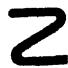
\includegraphics[keepaspectratio]{images/part001_10033d49.jpg}}

既开又闭的集合含有其每一点的分支，由此，一点的分支含于既开又闭且含有该点的诸集合之交。然而，一点的分支未必等于这个交（参见习题 9 及第二章，§ 4，第 4 目，命题 6）。

命题 9. 拓扑空间 X 中任一点的分支是闭集。关系“y 属于 x 的分支”是 X 上的一个等价关系 R\{x, y\}，其等价类就是 X 的诸分支。商空间 X/R 是全不连通的。

命题的第一部分是定义 3 与连通集的闭包连通（第 1 目，命题 1）这一事实的直接推论。由于有公共点的诸连通集之并是连通的（第 1 目，命题 2），关系 R 是传递的，因而是等价关系（因为它显然是自反且对称的），且 x 关于 R 的等价类就是 x 的分支。尚须证明 X/R 是全不连通的。设 \(f: X \to X/R\) 是典范映射，F 是 X/R 中含有至少两个不同点的闭集；F 的逆像 \(\overline{f}^{1}(F)\) 在 X 中是闭的、关于 R 是饱和的，且含有 X 的至少两个不同分支，因而不连通。于是存在 X 中两个非空闭集 B, C，使得 \(B \cap C = \varnothing\) 且 \(B \cup C = \overline{f}^{1}(F)\)。\(\overline{f}^{1}(F)\) 中任一点 x 在 \(\overline{f}^{1}(F)\) 中的分支与 x 在 X 中的分支相同（由 R 的定义），因此在 \(\overline{f}^{1}(F)\) 中既开又闭的 B 与 C 关于 R 是饱和的。于是 \(f(B)\) 与 \(f(C)\) 在 X/R 中是闭的，且 \(f(B) \cup f(C) = F\)，\(f(B) \cap f(C) = \varnothing\)；这表明 F 不连通，从而 X/R 是全不连通的。

命题 10. 在积空间 \(\mathbf{X} = \prod_{i\in J}\mathbf{X}_i\) 中，\(x = (x_i)\) 在 \(\mathbf{X}\) 中的分支是诸 \(x_i\) 在因子 \(\mathbf{X}_i\) 中的分支之积。

这个积集合是连通的（第 4 目，命题 8）。反之，若 A 是 X 的含有 x 的连通子集，则 \(\mathrm{pr}_{i}(A)\) 是含有 x 的连通集（第 2 目，命题 4）；由于 \(A \subset \prod_{i} \mathrm{pr}_{i}(A)\)，可见 A 含于诸 \(x_{i}\) 的分支之积中。

\subsection{局部连通空间}

定义 4. 如果拓扑空间 X 的每一点都有一个由连通邻域组成的基本邻域系，就称 X 为局部连通的。

* 我们将在第四章，§ 2，第 5 目看到，实直线是局部连通空间。*

在空间 X 的每点 x 处存在一个连通邻域，绝不能推出 X 是局部连通的。特别地，X 可以连通而非局部连通（习题 2 与 13）。反之，空间可以局部连通而不连通（例如含有多于一个点的离散空间）。

命题 11. 空间 X 局部连通的必要充分条件是：X 中开集的每个分支在 X 中都是开的。

该条件是充分的，因为这时 x 相对于 x 的一个开邻域的分支是 x 在 X 中的一个邻域。

反之，设 A 是局部连通空间 X 的开子集，B 是 A 的一个分支，且设 \(x \in B\)。设 V 是包含于 A 中的 x 的一个连通邻域；由分支的定义，V 含于 B；故 B 在 X 中是开的（§ 1，第 2 目，命题 1）。

因此，局部连通空间 X 的诸分支构成 X 的一个分成开集的分拆，从而 X 是它的诸分支的和（§ 2，第 4 目，例 3）。

推论. 设 U 是局部连通空间 X 的开子集，V 是 U 的一个分支。则 V 的边界（相对于 X）含于 U 的边界。

因为 V 在 U 中既开又闭，故 V 的边界点（相对于 X）不能属于 U，否则它也将是 V 相对于 U 的边界点，而这样的点不存在。

命题 12. 局部连通空间的每个商空间都是局部连通的。

设 X 是局部连通空间，R 是 X 上的等价关系，\(\varphi: X \to X/R\) 是典范映射。设 A 是

X/R 的一个开子集，C 是 A 的一个分支。则 \(\overline{\varphi}^{1}(C)\) 是 \(\overline{\varphi}^{1}(A)\) 的诸分支之并；因为若 \(x \in \overline{\varphi}^{1}(C)\)，且 K 是 \(x\) 在 \(\overline{\varphi}^{1}(A)\) 中的分支，则 \(\varphi(K)\) 是连通的（第 2 目，命题 4），含于 A，且含有 \(\varphi(x)\)；于是由 C 的定义有 \(\varphi(K) \subset C\)，因此 \(K \subset \overline{\varphi}^{1}(C)\)。既然 X 局部连通而 \(\overline{\varphi}^{1}(A)\) 在 X 中是开的，由命题 11 得 \(\overline{\varphi}^{1}(C)\) 在 X 中是开的；从而 C 在 X/R 中是开的，故再由命题 11，X/R 是局部连通的。

命题 13. a) 设 \((\mathbf{X}_t)_{t \in I}\) 是局部连通空间的一个族，使得 \(\mathbf{X}_t\) 除有限多个指标 \(t \in I\) 外都是连通的。则积空间 \(\mathbf{X} = \prod_{i \in I} \mathbf{X}_t\) 是局部连通的。

\begin{enumerate}
\def\labelenumi{\alph{enumi})}
\setcounter{enumi}{1}
\item
  反之，若非空拓扑空间的族 \((\mathbf{X}_{t})\) 之积是局部连通的，则每个 \(X_{t}\) 都局部连通，且 \(X_{t}\) 除有限多个指标外都连通。
\item
  设 \(\mathbf{J}\) 是 \(\mathbf{I}\) 的有限子集，使得 \(\mathbf{X}_i\) 不连通当且仅当 \(i \in \mathbf{J}\)。设
\end{enumerate}

\[
\mathrm{U} = \prod_ {i \in I} \mathrm{U} _ {i}
\]

是含有一点 \(x = (x_{t})\)（属于 \(\mathbf{X}\)）的初等集，并设 \(\mathbf{K}\) 是 \(\mathbf{I}\) 的有限子集，使得 \(\mathbf{U}_{t} \neq \mathbf{X}_{t}\) 当且仅当 \(t \in \mathbf{K}\)。令 \(\mathbf{V}_{t}\) 为 \(\mathbf{X}_{t}\)（当 \(t \notin J \cup K\)），而令 \(V_{t}\) 为 \(x_{t}\) 的一个含于 \(U_{t}\) 中的连通邻域（当 \(t \in J \cup K\)）；则

\[
\mathbf {V} = \prod_ {i \in I} \mathbf {V} _ {i}
\]

是连通的（由第 4 目命题 8），且是包含于 U 中的 x 的一个邻域。故 X 局部连通。

\begin{enumerate}
\def\labelenumi{\alph{enumi})}
\setcounter{enumi}{1}
\tightlist
\item
  设 \(a = (a_{i})\) 是 \(\mathbf{X}\) 的一点，\(\mathbf{V}\) 是 \(a\) 在 \(\mathbf{X}\) 中的一个连通邻域。由于除有限多个指标外有 \(\mathrm{pr}_{\mathfrak{i}}\mathbf{V} = \mathbf{X}_{\mathfrak{i}}\)（§ 4，第 1 目），由第 2 目命题 4，诸 \(\mathbf{X}_{\mathfrak{i}}\) 除有限多个指标外都是连通的。另一方面，对每个 \(x \in I\)、每个 \(a_{x} \in X_{x}\) 以及邻域 \(V_{x}\)（即 \(a_{x}\) 在 \(X_{x}\) 中的邻域），存在一点 \(x\)（属于 \(\mathbf{X}\)）使得 \(\mathrm{pr}_{\mathfrak{x}}x = a_{x}\)，且
\end{enumerate}

\[
\mathbf {V} = \mathbf {V} _ {x} \times \prod_ {i \neq x} \mathbf {X} _ {i}
\]

是 \(x\) 在 \(\mathbf{X}\) 中的一个邻域；于是 \(\mathbf{V}\) 含有一个连通邻域 \(W\)（即 \(x\) 的连通邻域），其投影 \(\mathrm{pr}_xW\) 是 \(a_x\) 的一个连通邻域，且含于 \(V_x\) 中（第 2 目，命题 4 及 § 4，第 2 目，命题 5）。故每个 \(X_x\) 都局部连通。

\subsection{应用：Poincaré-Volterra 定理}

定理 1. 设 X 是满足公理 (O \(_{III}\) )（但不一定是豪斯多夫的）的拓扑空间，且设 X 连通且局部连通。设 Y 是拓扑具有可数基的拓扑空间，p: X → Y 是连续映射，使得对每个 y ∈ Y，\(\overline{p}^{1}(y)\) 是 X 的离散子空间。最后设 B 是由 X 的子集组成的一个集，其诸成员的内部覆盖 X，且满足：

\begin{enumerate}
\def\labelenumi{(\roman{enumi})}
\tightlist
\item
  \(p\) 在每个 \(V \in \mathfrak{B}\) 上的限制是 \(V\) 到 \(Y\) 中的一个闭映射。\\
\item
  每个 \(V \in \mathfrak{B}\) 都有一个在 \(V\) 中稠密的可数子集。
\end{enumerate}

则空间 X 是一个可数开集族之并，其中每个开集都含于 B 的某个集合中。

设 \(\mathfrak{B}\) 是 Y 的拓扑的一个可数基。我们称一对 (W, U) 是特异的，如果 (i) \(U \in \mathfrak{B}\)，且 (ii) W 是 \(\overline{p}(U)\) 的一个分支，它含于 \(\mathfrak{B}\) 的某个集合中。

引理 1. 若 \(x\) 是 \(\mathbf{X}\) 的任一点，则存在特异对 \((\mathbf{W}, \mathbf{U})\) 使得 \(x \in \mathbf{W}\)。

逆像 \(\overline{p} (p(x))\) 是离散的，因而存在 \(x\) 在 \(\mathbf{X}\) 中的一个邻域，使得对其每一点 \(x^{\prime}\)（异于 \(x\) 者）都有像 \(p(x^{\prime})\neq p(x)\)；由于 \(\mathbf{X}\) 满足 \((\mathrm{O}_{\mathrm{III}})\)，存在具有该性质的闭邻域 \(\mathbf{V}\)（即 \(x\) 的闭邻域），且还可假设 \(\mathbf{V}\) 含于 \(\mathfrak{B}\) 的某个集合中。设 \(\mathbf{F}\) 是 \(\mathbf{V}\) 在 \(\mathbf{X}\) 中的边界。由定理的条件 (i)，\(p(\mathbf{F})\) 在 \(\mathbf{Y}\) 中是闭的；且由于 \(p(\mathbf{F})\) 不含 \(p(x)\)，存在集合 \(\mathbf{U}\in \mathfrak{B}\)，它含有 \(p(x)\) 且不与 \(p(\mathbf{F})\) 相交。设 \(\mathbf{W}\) 是 \(x\) 在 \(\overline{p}^{1}(\mathbf{U})\) 中的分支；则只须证明 \(\mathbf{W}\subset \mathring{\mathbf{V}}\)。若不然，\(\mathbf{W}\) 将与 \(\mathbf{F}\) 相交（第 1 目，命题 3），因而 \(p(\mathbf{F})\) 将与 \(\mathbf{U}\) 相交，这与 \(\mathbf{U}\) 的定义相矛盾。

引理 2. 若 (W, U) 是一个特异对，则使 W' 与 W 相交的所有特异对 (W', U') 所成的集是可数的。

既然 \(\mathfrak{B}\) 是可数的，只须证明：对给定的 \(\mathbf{U}' \in \mathfrak{B}\)，特异对 \((\mathbf{W}', \mathbf{U}')\)（其中 \(\mathbf{W}'\) 与 \(\mathbf{W}\) 相交者）所成的集是可数的。现在这些集合 \(\mathbf{W}'\) 都是开的，因为 \(\mathbf{X}\) 局部连通（第 6 目，命题 11），且两两不相交，因为它们是 \(\overline{\boldsymbol{p}}(\mathbf{U}')\) 的分支；于是诸集合 \(\mathbf{W}' \cap \mathbf{W}\) 是开的且两两不相交。但 \(\mathbf{W}\) 含有一个在 \(\mathbf{W}\) 中稠密的可数子集；故诸 \(\mathbf{W}'\)（其中 \(\mathbf{W}' \cap \mathbf{W}\) 非空者）所成的集也是可数的。

为证定理 1，考虑 X 的两点 \(x\), \(x'\) 之间的如下关系 R：“存在特异对的一个有限序列 \((W_i, U_i)\)（\(1 \leqslant i \leqslant n\)），使得 \(x \in W_1\)，\(x' \in W_n\)，且 \(W_i \cap W_{i+1} \neq \emptyset\) 对 \(1 \leqslant i \leqslant n - 1\) 成立。”

引理 1 表明 R 是自反的，且容易验证 R 是对称且传递的，故 R 是一个等价关系；又由于诸 \(W_{i}\) 是开的，每个模 R 等价类都在 X 中是开的。但 X 连通；故只能有一个等价类，即 X 的任意两点都模 R 同余。我们将由此推出，X 是特异对第一元素所成的一个可数族之并，这就证明了定理 1。为此，设 x 是 X 的任一点，并对 n 用归纳法定义 X 的开子集的序列 \((\mathbf{C}_{n})\) 如下：由引理 1，存在特异对 \((\mathbf{W}_{1}, \mathbf{U}_{1})\) 使得 \(x \in W_{1}\)，我们取 \(C_{1} = W_{1}\)；若 n \textgreater{} 1，则 \(C_{n}\) 取为所有使 W 与 \(C_{n-1}\) 相交的特异对 (W, U) 的第一元素 W 的并。由引理 2，对 n 用归纳法立即可见，\(C_{n}\) 是特异对第一元素的一个可数并。最后，每个 \(x' \in X\) 都属于某个 \(C_{n}\)；因为存在有限序列

\[
\left(\mathrm{W} _ {i} ^ {\prime}, \mathrm{U} _ {i} ^ {\prime}\right) _ {1 \leqslant i \leqslant m}
\]

的特异对，使得 \(x \in W_1'\)，\(x' \in W_m'\)，且 \(W_i' \cap W_{i+1}' \neq \emptyset\) 对 \(1 \leqslant i \leqslant m - 1\) 成立；对 \(i\) 用归纳法可以看出，\(W_i' \subset C_{i+1}\) 对所有 \(i\) 都成立，从而 \(x' \in C_{m+1}\)。

证毕。

推论 1. 设 Y 是拓扑具有可数基的正则空间（*）。设 X 是连通且局部连通的空间，且设 \(p: \mathbf{X} \to \mathbf{Y}\) 是具有以下性质的连续映射：对每个 \(x \in \mathbf{X}\)，存在 \(x\) 在 X 中的一个闭邻域 V，使得 \(p\) 在 V 上的限制是 V 到 Y 的一个闭子空间上的同胚。则 X 是正则的且 X 的拓扑具有可数基。

首先，诸假设蕴含 X 是正则的（§ 8，第 4 目，命题 13）。让我们证明，若取 B 为 X 的所有这样的闭子集 V 所成的集：p 在 V 上的限制是 V 到 Y 的一个闭子空间上的同胚，则定理 1 的条件得到满足。按假设，B 中诸集合的内部覆盖 Y，且凭关于 Y 的假设，每个 \(V \in B\) 都具有可数基，因而含有一个可数稠密子集（§ 1，第 6 目，命题 6）。此外，若 \(x \in \overline{p}(y)\)，则存在 x 在 X 中的一个邻域 \(V \in B\)，使得 V 不含 \(\overline{p}(y)\) 的异于 \(x\) 的任何点，从而 \(\overline{p}(y)\) 是一个离散空间。于是可以应用定理 1，它表明 X 是开集的一个可数族 \((\mathrm{T}_n)_{n\geqslant 0}\) 之并，使得每个子空间 \(\mathrm{T}_n\) 都具有可数基 \((\mathrm{U}_{mn})_{m\geqslant 0}\)。于是诸 \(\mathrm{U}_{mn}\)（\(m\geqslant 0\)，\(n\geqslant 0\)）构成 X 的拓扑的一个基（§ 3，第 1 目，注）。

推论 2. 设 X 局部紧、连通且局部连通，并设 X 的每一点都有一个具有可数基的邻域。设 Y 是拓扑具有可数基的豪斯多夫空间，且设 \(p: \mathbf{X} \to \mathbf{Y}\) 是连续映射，使得对每个 \(y \in \mathbf{Y}\)，\(\overline{p}^1(y)\) 是 X 的离散子空间。则 X 的拓扑具有可数基。

对每个 \(x \in X\)，设 \(V_{x}\) 是 x 在 X 中的一个具有可数基的紧邻域。由 §9，第 4 目，定理 2，推论 2 可知，诸 \(V_{x}\) 所成的集 B 满足定理 1 的条件，于是我们像推论 1 中那样完成证明。

注意，在此推论中，可能发生这样的情形：p 在 X 的某一点的任意小邻域 V 上的限制不是 V 到 \(p(\mathrm{V})\) 上的同胚。

推论 3（Poincaré-Volterra 定理）. 设 Y 是局部紧、局部连通且拓扑具有可数基的空间。设 X 是连通豪斯多夫空间，且设 \(p: \mathbf{X} \to \mathbf{Y}\) 是具有以下性质的连续映射：对每个 \(x \in \mathbf{X}\)，存在 \(x\) 在 X 中的一个开邻域 U，使得 \(p\) 在 U 上的限制是 U 到 Y 的一个开子空间上的同胚。则 X 局部紧且局部连通，且 X 的拓扑具有可数基。

显然 X 局部连通。又每个 \(x \in X\) 都有 X 中的一个开邻域 U，使得 p 在 U 上的限制把 U 同胚地映到 Y 的开子空间 \(p(U)\) 上。由于 \(p(U)\) 是 Y 的局部紧子空间（\(§ 9, no. 7, Proposition 13\)），存在 \(p(x)\) 的一个紧邻域 W，它含于 \(p(U)\) 中，从而 \(U \cap \overline{p}(W)\) 是含于 U 中的 x 的一个紧邻域；由于按假设 X 是豪斯多夫的，故 X 局部紧。\(U \cap \overline{p}(W)\) 是紧的，故在 X 中是闭的（\(§ 9, no. 3, Proposition 4\)），因而推论 1 的条件得到满足；故 X 的拓扑具有可数基。

\BourbakiExercises
\BourbakiExerciseGroup

\begin{enumerate}
\def\labelenumi{\arabic{enumi})}
\item
  求出两个元素的集合或三个元素的集合上的所有可能的拓扑。
\item
  \begin{enumerate}
  \def\labelenumii{\alph{enumii})}
  \tightlist
  \item
    设 X 是一个有序集。证明区间所成的集
  \end{enumerate}
\end{enumerate}

\[
[ x, \rightarrow [ \quad (\text { resp. } ] \leftarrow , x ])
\]

是 X 上一个拓扑的基；这一拓扑称为 X 的右拓扑（相应地，左拓扑）。在右拓扑中，开集的任意交是开集，且 \(\{x\}\) 的闭包是区间 {]}\(\leftarrow\), x{]}。

\begin{enumerate}
\def\labelenumi{\alph{enumi})}
\setcounter{enumi}{1}
\item
  若拓扑空间满足以下条件，则称它为 Kolmogoroff 空间：给定任意两个不同的点 \(x\), \(x'\)（属于 \(X\)），存在这两点之一的一个邻域，它不含另一点。证明带有右拓扑的有序集是 Kolmogoroff 空间。
\item
  设 X 是一个 Kolmogoroff 空间，其中开集的每个交都是开集。证明 \(x \in \overline{\{x'\}}\) 是 X 中 x 与 \(x'\) 之间的一个序关系，且若把这个关系记作 \(x \leqslant x'\)，则 X 上给定的拓扑与由这个排序所确定的右拓扑相同。
\item
  由 c) 推出：若 X 是 Kolmogoroff 空间，则 X 的每个有限非空子集至少有一个孤立点。因此，若 X 没有孤立点，则 X 的每个非空开子集都是无限的。
\end{enumerate}

\begin{enumerate}
\def\labelenumi{\arabic{enumi})}
\setcounter{enumi}{2}
\tightlist
\item
  若 \(\mathbf{A}\) 是拓扑空间 \(\mathbf{X}\) 的任一子集，用 \(\alpha(\mathbf{A})\) 表示 \(\overline{\mathbf{A}}\)，用 \(\beta(\mathbf{A})\) 表示 \(\overline{\mathbf{A}}\)。则 \(\mathbf{A} \subset \mathbf{B}\) 蕴含 \(\alpha(\mathbf{A}) \subset \alpha(\mathbf{B})\) 与 \(\beta(\mathbf{A}) \subset \beta(\mathbf{B})\)。\(a)\) 证明：若 \(\mathbf{A}\) 是开的，则 \(\mathbf{A} \subset \alpha(\mathbf{A})\)；若 \(\mathbf{A}\) 是闭的，则 \(\beta(\mathbf{A}) \subset \mathbf{A}\)。
\end{enumerate}

\begin{enumerate}
\def\labelenumi{\alph{enumi})}
\setcounter{enumi}{1}
\item
  由 a) 推出：若 A 是 X 的任一子集，则 \(\alpha(\alpha(A)) = \alpha(A)\) 且 \(\beta(\beta(A)) = \beta(A)\)。
\item
  给出集合 A 的一个例子 \(*\)（在实直线上）\(_{*}\)，使得七个集合 A、\(\mathring{A}\)、\(\overline{A}\)、\(\alpha(A)\)、\(\beta(A)\)、\(\beta(\overline{A})\)、\(\alpha(\mathring{A})\) 两两不同，且除以下关系外不满足任何包含关系：\(\mathring{A} \subset A \subset \overline{A}\)，\(\mathring{A} \subset \alpha(\mathring{A}) \subset \beta(A) \subset \overline{A}\)，\(\mathring{A} \subset \alpha(A) \subset \beta(\overline{A}) \subset \overline{A}\)，\(\alpha(\mathring{A}) \subset \alpha(A)\)，\(\beta(A) \subset \beta(\overline{A})\)。
\item
  证明：若 U, V 是两个开集，使得 \(U \cap V = \varnothing\)，则也有 \(\alpha(U) \cap \alpha(V) = \varnothing\) {[}用 b){]}。
\end{enumerate}

\begin{enumerate}
\def\labelenumi{\arabic{enumi})}
\setcounter{enumi}{3}
\tightlist
\item
  \begin{enumerate}
  \def\labelenumii{\alph{enumii})}
  \tightlist
  \item
    在实直线上给出两个开集 A, B 的一个例子 *（在实直线上）*，使得四个集合 A ∩ B、B ∩ A̅、A ∩ B 与 A̅ ∩ B 两两不同。
  \end{enumerate}
\end{enumerate}

\begin{enumerate}
\def\labelenumi{\alph{enumi})}
\setcounter{enumi}{1}
\tightlist
\item
  * 在实直线上给出两个区间 A, B 的一个例子，使得 A ∩ B 不含于 A ∩ B。*
\end{enumerate}

\begin{enumerate}
\def\labelenumi{\arabic{enumi})}
\setcounter{enumi}{4}
\tightlist
\item
  若 A 是拓扑空间 X 的任一子集，A 的边界记作 \(\operatorname{Fr}(\mathbf{A})\)。
\end{enumerate}

\begin{enumerate}
\def\labelenumi{\alph{enumi})}
\item
  证明 \(\operatorname{Fr}(\overline{\mathbf{A}}) \subset \operatorname{Fr}(\mathbf{A})\)，\(\operatorname{Fr}(\mathring{\mathbf{A}}) \subset \operatorname{Fr}(\mathbf{A})\)，并给出一个例子 *（在实直线上）*，其中这三个集合两两不同。
\item
  设 A, B 是 X 的两个子集；证明
\end{enumerate}

\[
\operatorname{Fr} (\mathbf {A} \cup \mathbf {B}) \subset \operatorname{Fr} (\mathbf {A}) \cup \operatorname{Fr} (\mathbf {B})
\]

并给出一个例子 *（在实直线上）*，其中这些集合两两不同。若 \(\overline{\mathbf{A}} \cap \overline{\mathbf{B}} = \emptyset\)，证明 \(\operatorname{Fr}(\mathbf{A} \cup \mathbf{B}) = \operatorname{Fr}(\mathbf{A}) \cup \operatorname{Fr}(\mathbf{B})\)。

\begin{enumerate}
\def\labelenumi{\alph{enumi})}
\setcounter{enumi}{2}
\tightlist
\item
  若 \(\mathbf{A}\) 与 \(\mathbf{B}\) 在 \(\mathbf{X}\) 中是开的，证明
\end{enumerate}

\[
\begin{array}{r l} & (\mathbf {A} \cap \operatorname{Fr} (\mathbf {B})) \cup (\mathbf {B} \cap \operatorname{Fr} (\mathbf {A})) \subset \operatorname{Fr} (\mathbf {A} \cap \mathbf {B}) \\ & \qquad \subset (\mathbf {A} \cap \operatorname{Fr} (\mathbf {B})) \cup (\mathbf {B} \cap \operatorname{Fr} (\mathbf {A})) \cup (\operatorname{Fr} (\mathbf {A}) \cap \operatorname{Fr} (\mathbf {B})) \end{array}
\]

并给出一个例子 *（在实直线上）*，其中这三个集合两两不同。

\begin{enumerate}
\def\labelenumi{\arabic{enumi})}
\setcounter{enumi}{5}
\item
  证明：拓扑空间 X 的子集 A 与 X 的每个稠密子集相交，当且仅当 A 的内部非空。
\item
  考虑给定拓扑空间 \(\mathbf{X}\) 的以下四个性质：
\end{enumerate}

(D \(_{I}\) ) X 的拓扑具有可数基。

\((D_{II})\) X 有一个可数稠密子集。

\((D_{III})\) X 的每个所有点都是孤立点的子集是可数的。

\((D_{IV})\) X 的两两不相交的非空开子集所成的每个集是可数的。

证明 \((\mathbf{D}_{\mathbf{I}})\) 蕴含 \((\mathbf{D}_{\mathbf{II}})\) 与 \((\mathbf{D}_{\mathbf{III}})\)，且 \((\mathbf{D}_{\mathbf{II}})\) 与 \((\mathbf{D}_{\mathbf{III}})\) 各自蕴含 \((\mathbf{D}_{\mathbf{IV}})\)（*）。

\begin{enumerate}
\def\labelenumi{\arabic{enumi})}
\setcounter{enumi}{7}
\item
  若拓扑空间 X 的子集 A 没有孤立点，则它在 X 中的闭包 \(\overline{A}\) 也没有孤立点。
\item
  设 X 是一个集合，\(M \to \overline{M}\) 是 \(\mathfrak{P}(X)\) 到其自身上的一个映射，使得：1) \(\overline{\varnothing} = \varnothing\)；2) 对每个 \(M \subset X\) 有 \(M \subset \overline{M}\)；3) 对每个 \(M \subset X\) 有 \(\overline{M} = \overline{M}\)；4) 对所有 \(M \subset X\) 与 \(N \subset X\) 有
\end{enumerate}

\[
\overline {{\mathbf {M} \cup \mathbf {N}}} = \overline {{\mathbf {M}}} \cup \overline {{\mathbf {N}}}.
\]

证明 X 上存在唯一的拓扑，使得 \(\overline{M}\)（对所有 \(M \subset X\)）是 M 关于这个拓扑的闭包（借助其闭集来定义这个拓扑）。

\BourbakiExerciseGroup

\begin{enumerate}
\def\labelenumi{\arabic{enumi})}
\tightlist
\item
  设 \(f\) 是拓扑空间 \(\mathbf{X}\) 到拓扑空间 \(\mathbf{X}'\) 中的一个映射。证明以下命题等价：
\end{enumerate}

\begin{enumerate}
\def\labelenumi{\alph{enumi})}
\item
  \(f\) 在 \(\mathbf{X}\) 上是连续的。
\item
  对每个子集 \(\mathbf{A}'\)，有 \(\mathbf{X}', f^1 (\mathring{\mathbf{A}}') \subset (f^1 (\mathbf{A}'))^0\)。
\item
  对每个子集 \(\mathbf{A}'\)，有 \(\mathbf{X}', \overline{f}^1 (\mathbf{A}') \subset \overline{f}^1 (\overline{\mathbf{A}}')\)。
\end{enumerate}

用一个例子证明：若 \(f\) 连续，集合 \(\overline{f}^1 (\mathbf{A}')\) 与 \(\overline{f}^1 (\overline{\mathbf{A}}')\) 仍可以不同。

\begin{enumerate}
\def\labelenumi{\arabic{enumi})}
\setcounter{enumi}{1}
\item
  设 X, X' 是两个有序集，各赋予右拓扑（§ 1，习题 2）。证明映射 \(f: \mathbf{X} \to \mathbf{X}'\) 连续当且仅当它是保序的。
\item
  设 X, X' 是两个拓扑空间，f 是 X 到 X' 上的一个双射；则 f 是 X 到 \(X'\) 上的同胚的必要充分条件是：\(X'\) 的拓扑是使 f 连续的最细拓扑。
\item
  在有序集 X 上，左拓扑与右拓扑（§ 1，习题 2）的上确界是离散拓扑；若 X 是有向集（向右或向左有向），则这两个拓扑的下确界是 X 上最粗的拓扑。
\item
  在有序集 X 上，用 \(\mathcal{C}_{0}(\mathbf{X})\)（相应地，\(\mathcal{C}_{+}(\mathbf{X})\)，\(\mathcal{C}_{-}(\mathbf{X})\)）表示由所有开区间（相应地，右半开区间所成的集、左半开区间所成的集）生成的拓扑，这些区间可以有界也可以无界。
\end{enumerate}

\begin{enumerate}
\def\labelenumi{\alph{enumi})}
\item
  证明：若 X 是线性序的，则开（相应地，右半开、左半开）区间构成 \(\mathcal{C}_{0}(\mathbf{X})\)（相应地，\(\mathcal{C}_{+}(\mathbf{X})\)，\(\mathcal{C}_{-}(\mathbf{X})\)）的一个基；且闭区间在这三个拓扑的每一个中都是闭集。
\item
  在线性序集 X 上，证明拓扑 \(\mathcal{C}_{+}(\mathbf{X})\) 比右拓扑（§ 1，习题 2）细，拓扑 \(\mathcal{C}_{-}(\mathbf{X})\) 比左拓扑细，且拓扑 \(\mathcal{C}_{0}(\mathbf{X})\) 是 \(\mathcal{C}_{+}(\mathbf{X})\) 与 \(\mathcal{C}_{-}(\mathbf{X})\) 的交。
\item
  设 X 是一个线性序集。证明 \(\mathfrak{C}_{0}(\mathbf{X})\) 具有可数基的必要充分条件是：存在 X 的一个可数子集 D，使得对每个 \(x \in X\) 以及每个含有 x 的区间 {]}a, b{[}，存在 \(\alpha \in D\) 与 \(\beta \in D\) 使得
\end{enumerate}

\[
a \leqslant \alpha <   x <   \beta \leqslant b
\]

{[}参见第四章，§ 2，习题 11 c){]}。

\begin{enumerate}
\def\labelenumi{\alph{enumi})}
\setcounter{enumi}{3}
\tightlist
\item
  证明：若 X 是良序的（《集合论》，第三章，§ 2），则拓扑 \(\mathcal{G}_{+}(\mathbf{X})\) 是离散拓扑，且拓扑 \(\mathcal{G}_{0}(\mathbf{X})\) 与 \(\mathcal{G}_{-}(\mathbf{X})\) 相同。
\end{enumerate}

¶ 6) 集合 X 上的一个拓扑称为拟极大的，如果它在使 X 没有孤立点的诸拓扑所成的集中是极大的。

\begin{enumerate}
\def\labelenumi{\alph{enumi})}
\item
  证明 X 上的拓扑 \(\mathcal{G}\) 的以下性质等价：\(\alpha\) \(\mathcal{G}\) 是拟极大的；\(\beta\) 若 X 带有拓扑 \(\mathcal{G}\)，则 X 没有孤立点，且 X 的每个没有孤立点的子集都是开的。
\item
  设 X 是一个 Kolmogoroff 空间（§ 1，习题 2），其中每个非空开集都是无限的。证明 X 上存在一个比给定拓扑更细的拟极大拓扑（证明 X 上使所有非空开集都是无限的诸拓扑所成的集是归纳的，并用 § 1 的习题 2 d)）。
\end{enumerate}

\begin{enumerate}
\def\labelenumi{\arabic{enumi})}
\setcounter{enumi}{6}
\tightlist
\item
  若 X 是任一集合，用 \(\mathfrak{P}_{0}(\mathbf{X})\) 表示 X 的非空子集所成的集。
\end{enumerate}

\begin{enumerate}
\def\labelenumi{\alph{enumi})}
\item
  设 X 是一个非空拓扑空间。用 \(\mathcal{G}_{\Omega}\)（相应地，\(\mathcal{G}_{\Phi}\)）表示 \(\mathfrak{P}_{0}(\mathbf{X})\) 上使下列条件成立的最粗拓扑：对 X 的每个非空开（相应地，闭）子集 A，\(\mathfrak{P}_{0}(\mathbf{A})\) 在 \(\mathfrak{P}_{0}(\mathbf{X})\) 中是开的（相应地，闭的）。证明这两个拓扑一般不可比较，且映射 \(x \to \{x\}\) 是 X 到 \(\mathfrak{P}_{0}(\mathbf{X})\) 的一个子空间上的同胚，只要后一集合带有拓扑 \(\mathcal{G}_{\Omega}, \mathcal{G}_{\Phi}\) 之一。
\item
  设 D 是 X 的一个稠密子集。证明 D 的有限非空子集所成的集 \(\mathfrak{E}(D)\) 在 \(\mathfrak{P}_{0}(X)\) 中对于拓扑 \(C_{\Omega}, C_{\Phi}\) 中的每一个都是稠密的。
\item
  若 \(\mathfrak{P}_{0}(\mathbf{X})\) 按包含关系排序，证明拓扑 \(\mathcal{C}_{\Omega}\) 比 \(\mathfrak{P}_{0}(\mathbf{X})\) 上的左拓扑（\(\S\) 1，习题 2）粗；\(\mathbf{A} \in \mathfrak{P}_{0}(\mathbf{X})\) 在拓扑 \(\mathcal{C}_{\Omega}\) 中是孤立点，当且仅当 \(\mathbf{A} = \{x\}\)（其中 \(x\) 是 \(\mathbf{X}\) 的一个孤立点）；且 \(\mathbf{A} \in \mathfrak{P}_{0}(\mathbf{X})\) 在拓扑 \(\mathcal{C}_{\Phi}\) 中是孤立点，当且仅当 \(\mathbf{X}\) 是有限离散空间且 \(\mathbf{A} = \mathbf{X}\)。
\item
  证明：若 \(\mathfrak{P}_0(\mathbf{X})\) 带有拓扑 \(\mathcal{C}_{\Omega}\)（相应地，\(\mathcal{C}_{\Phi}\)）且
\end{enumerate}

\[
\mathfrak {P} _ {\mathbf {0}} (\mathbf {X}) \times \mathfrak {P} _ {\mathbf {0}} (\mathbf {X})
\]

带有 \(\mathcal{C}_{\Omega}\)（相应地，\(\mathcal{C}_{\Phi}\)）与其自身的积拓扑，则映射 \((\mathbf{M}, \mathbf{N}) \to \mathbf{M} \cup \mathbf{N}\)（\(\mathfrak{P}_0(\mathbf{X}) \times \mathfrak{P}_0(\mathbf{X})\) 到 \(\mathfrak{P}_0(\mathbf{X})\) 中的映射）是连续的。

\begin{enumerate}
\def\labelenumi{\alph{enumi})}
\setcounter{enumi}{4}
\tightlist
\item
  证明：若 \(\mathfrak{P}_{0}(\mathbf{X})\) 带有拓扑 \(\mathfrak{T}_{\Phi}\)，则映射 \(\mathbf{M} \to \overline{\mathbf{M}}\) 是连续的。
\end{enumerate}

\(f)\) 设 \(\mathbf{X}\), \(\mathbf{Y}\) 是两个拓扑空间，\(f: \mathbf{X} \to \mathbf{Y}\) 是连续映射。证明：若 \(\mathfrak{P}_{0}(\mathbf{X})\) 与 \(\mathfrak{P}_{0}(\mathbf{Y})\) 都带有拓扑 \(\mathcal{G}_{\Omega}\)，且都带有拓扑 \(\mathcal{G}_{\Phi}\)，则映射 \(\mathbf{M} \to f(\mathbf{M})\)（\(\mathfrak{P}_{0}(\mathbf{X})\) 到 \(\mathfrak{P}_{0}(\mathbf{Y})\) 中的映射）是连续的。

\begin{enumerate}
\def\labelenumi{\alph{enumi})}
\setcounter{enumi}{6}
\tightlist
\item
  设 X, Z 是两个拓扑空间。证明：映射 \(f: Z \to \mathfrak{P}_{0}(X)\) 当 \(\mathfrak{P}_{0}(X)\) 带有拓扑 \(C_{\Omega}\)（相应地，\(C_{\Phi}\)）时连续的必要充分条件是：对 X 的每个闭（相应地，开）子集 A，由 \(z \in Z\)（满足 \(f(z) \cap A \neq \emptyset\) 者）全体所成的集在 Z 中是闭的（相应地，开的）。
\end{enumerate}

\begin{enumerate}
\def\labelenumi{\arabic{enumi})}
\setcounter{enumi}{7}
\tightlist
\item
  设 X 是一个集合，c 是一个基数，它或是无限或等于 1。由 X 与那些满足 card(M) \textless{} c 的 M ⊆ X 组成的 X 的子集所成的集，是 X 关于某个拓扑 \(\mathfrak{G}_{\mathfrak{c}}\) 的闭子集所成的集；\(\mathfrak{G}_{\mathfrak{1}}\) 是 X 上最粗的拓扑，而 \(\mathfrak{G}_{\mathfrak{c}}\) 在 c \textgreater{} card (X) 时是离散拓扑。X 的每个置换都是把 X 赋予拓扑 \(\mathfrak{G}_{\mathfrak{c}}\) 所得拓扑空间的一个自同构。
\end{enumerate}

证明反之，任何拓扑 \(\mathcal{C}\)（在 \(\mathbf{X}\) 上）若具有性质：\(\mathbf{X}\) 的每个置换关于 \(\mathcal{C}\) 都连续，则它必然是诸拓扑 \(\mathcal{C}_{\mathfrak{c}}\) 之一。{[}设 \(\mathfrak{c}\) 是使 card \((\mathbf{F}) < \mathfrak{c}\)（对每个闭子集 \(\mathbf{F} \neq \mathbf{X}\)，在拓扑 \(\mathcal{C}\) 中）成立的最小基数；注意当 \(\mathbf{X}\) 无限且 \(\mathfrak{c} >\mathrm{card}(\mathbf{X})\) 时，\(\mathcal{C}\) 必然是离散拓扑。{]}

\begin{enumerate}
\def\labelenumi{\arabic{enumi})}
\setcounter{enumi}{8}
\tightlist
\item
  \begin{enumerate}
  \def\labelenumii{\alph{enumii})}
  \tightlist
  \item
    在第 3 目命题 4 的假设下，证明 X 上使诸 \(f_{t}\) 连续的最粗拓扑也是 X 上具有以下性质的最细拓扑 \(\mathfrak{G}\)：从拓扑空间 Z 到 X 中的每个映射 \(g\)（使诸 \(f_{t} \circ g\) 连续者）都（关于 \(\mathfrak{G}\)）连续。
  \end{enumerate}
\end{enumerate}

\begin{enumerate}
\def\labelenumi{\alph{enumi})}
\setcounter{enumi}{1}
\tightlist
\item
  在第 4 目命题 6 的假设下，证明 X 上使诸 \(f_{i}\) 连续的最细拓扑也是 X 上具有以下性质的最粗拓扑 \(\mathcal{G}\)：从 X 到拓扑空间 Z 中的每个映射 \(g\)（使诸 \(g \circ f_{i}\) 连续者）都（关于 \(\mathcal{G}\)）连续。
\end{enumerate}

\begin{enumerate}
\def\labelenumi{\arabic{enumi}.}
\setcounter{enumi}{9}
\tightlist
\item
  在集合 X 上，设 M 是由没有孤立点的拓扑组成的一个有向集。证明 M 在 X 上所有拓扑所成的集中的上确界是一个没有孤立点的拓扑。
\end{enumerate}

¶ 11. 拓扑空间称为可解的，如果它是两个稠密子集的不相交并。

\begin{enumerate}
\def\labelenumi{\alph{enumi})}
\item
  若拓扑空间 X 可解，证明 X 没有孤立点，且 X 的每个开子空间都可解。再证明反之，若 X 是拓扑空间，B 是 X 的非空可解开子空间所成的一个集，使得 X 的每个非空开子集都含有属于 B 的一个集合，则 X 可解（考虑属于 B 的两两不相交开集的一个极大集）。
\item
  若 Kolmogoroff 空间 X 可解，则 X 的每个非空开子集都是无限的{[}用 §1 的习题 2d){]}。
\item
  设 X 是这样的拓扑空间：1) X 的非空开子集的最小基数 b 是无限的；2) X 的拓扑有一个基 B 使得 card (B) ≤ b。证明 X 可解。（用超限归纳法构造 X 的两个不相交稠密子集。）用《集合论》，第三章，§ 6，习题 24 a) 的方法。特别地，有理直线是可解的。
\item
  没有孤立点的拓扑空间 X 称为等势的，如果对 X 的每个非空开子集有 card (U) = card (X)。证明在一个没有孤立点的空间 X 中，X 的每个非空开集都含有一个非空的等势开子空间。由此推出，若 X 的每个等势开子空间都可解，则 X 可解。
\end{enumerate}

\BourbakiExerciseGroup

\begin{enumerate}
\def\labelenumi{\arabic{enumi})}
\tightlist
\item
  设 A, B 是拓扑空间 X 的两个子集，使得 \(A \supset B\)。证明：
\end{enumerate}

\begin{enumerate}
\def\labelenumi{\alph{enumi})}
\item
  B 相对于 X 的内部含于 B 相对于 X 的子空间 A 的内部。给出一个这两个集合不同的例子。
\item
  B 相对于 A 的边界含于 A 与 B 相对于 X 的边界之交。给出一个这两个集合不同的例子。
\end{enumerate}

\begin{enumerate}
\def\labelenumi{\arabic{enumi})}
\setcounter{enumi}{1}
\tightlist
\item
  设 A 与 B 是拓扑空间 X 的任意两个子集。
\end{enumerate}

\begin{enumerate}
\def\labelenumi{\alph{enumi})}
\item
  证明 A 与 B 相对于 X 的内部之交含于 \(B \cap A\) 相对于 A 的内部。给出一个这两个集合不同的例子。
\item
  证明 A 与 B 相对于 X 的闭包之交包含 B ∩ A 相对于 A 的闭包。给出一个这两个集合不同的例子。
\end{enumerate}

\begin{enumerate}
\def\labelenumi{\arabic{enumi})}
\setcounter{enumi}{2}
\item
  子空间 \(\mathbf{A}\)（属于拓扑空间 \(\mathbf{X}\)）是离散的，当且仅当 \(\mathbf{A}\) 的每一点都是孤立的。
\item
  设 Y, Z 是拓扑空间 X 的两个子空间，使得 \(X = Y \cup Z\)，且使得 \(\overline{A} \cap B = \overline{B} \cap A = \varnothing\)，其中 \(A = Y \cap CZ\)，\(B = Z \cap CY\)。
\end{enumerate}

\begin{enumerate}
\def\labelenumi{\alph{enumi})}
\item
  证明：若 M 是 X 的任一子集，则 M 在 X 中的闭包是 \(M \cap Y\) 在 Y 中的闭包与 \(M \cap Z\) 在 Z 中的闭包之并。由此推出，若 \(M \cap Y\) 在 Y 中是闭的（相应地，开的）且 \(M \cap Z\) 在 Z 中是闭的（相应地，开的），则 M 在 X 中是闭的（相应地，开的）。
\item
  设 \(f\) 是 \(\mathbf{X}\) 到拓扑空间 \(\mathbf{X}'\) 中的一个映射。证明：若 \(f|_{\mathbf{Y}}\) 与 \(f|_{\mathbf{Z}}\) 连续，则 \(f\) 也连续。
\end{enumerate}

\begin{enumerate}
\def\labelenumi{\arabic{enumi})}
\setcounter{enumi}{4}
\item
  设 Y, Z 是拓扑空间 X 的两个子空间，使得 \(X = Y \cup Z\)。证明：若 \(Y \cap Z\) 的子集 M 在 Y 与 Z 中都是开的（相应地，闭的），则 M 在 X 中是开的（相应地，闭的）。
\item
  设 A 是拓扑空间 X 的一个局部闭子空间。证明 X 的这样的开子集 U 所成的集——使得 \(A \subset U\) 且 A 在 U 中是闭的——有一个最大元素，即 A 相对于 \(\overline{A}\) 的边界在 X 中的余集。
\item
  用例子证明：两个局部闭子集的并与一个局部闭子集的余集未必是局部闭的。
\item
  设 A 是有序集 X 的一个子集。证明由 X 的右拓扑（相应地，左拓扑）（§ 1，习题 2）在 A 上诱导的拓扑，是 A 关于由 X 的序所诱导的 A 的序的右拓扑（相应地，左拓扑）。
\item
  设 \(\mathbf{A}\) 是线性序集 \(\mathbf{X}\) 的一个子集。
\end{enumerate}

\begin{enumerate}
\def\labelenumi{\alph{enumi})}
\item
  证明由拓扑 \(\mathcal{G}_{-}(\mathbf{X})\) {[}相应地 \(\mathcal{G}_{+}(\mathbf{X}),\mathcal{G}_{0}(\mathbf{X})]\)（§ 2，习题 5）在 A 上诱导的拓扑，比拓扑 \(\mathcal{G}_{-}(\mathbf{A})\) {[}相应地 \(\mathcal{G}_{+}(\mathbf{A}),\mathcal{G}_{0}(\mathbf{A})]\) 细，这里 A 的序是由 X 的序所诱导的序。若 A 是 X 的一个区间，则 \(\mathcal{G}_{-}(\mathbf{A})\) {[}相应地 \(\mathcal{G}_{+}(\mathbf{A}),\mathcal{G}_{0}(\mathbf{A})]\) 是由 \(\mathcal{G}_{-}(\mathbf{X})\) {[}相应地 \(\mathcal{G}_{+}(\mathbf{X}),\mathcal{G}_{0}(\mathbf{X})]\) 在 A 上诱导的拓扑。
\item
  取 X 为积 \(Q \times Z\)，按字典序排序（《集合论》，第三章，§ 2，第 6 目），并取 A 为子集 \(Q \times \{0\}\)。证明拓扑 \(\mathcal{G}_{-}(A)\) {[}相应地，\(\mathcal{G}_{+}(A)\)，\(\mathcal{G}_{0}(A)\){]} 严格地比由 \(\mathcal{G}_{-}(X)\) {[}相应地，\(\mathcal{G}_{+}(X)\)，\(\mathcal{G}_{0}(X)\){]} 在 A 上诱导的拓扑粗。
\end{enumerate}

\begin{enumerate}
\def\labelenumi{\arabic{enumi})}
\setcounter{enumi}{9}
\item
  设 A 是非空拓扑空间 X 的一个非空子空间。证明在 \(\mathfrak{P}_{0}(\mathbf{A})\) 上由拓扑 \(\mathcal{G}_{\Omega}\)（相应地，\(\mathcal{G}_{\Phi}\)）——\(\mathfrak{P}_{0}(\mathbf{X})\) 上的（§ 2，习题 7）——诱导的拓扑，就是拓扑 \(\mathcal{G}_{\Omega}\)（相应地，\(\mathcal{G}_{\Phi}\)）——\(\mathfrak{P}_{0}(\mathbf{A})\) 上的。
\item
  设 X 是拓扑空间，\(\mathcal{G}\) 是 X 的拓扑，A 是 X 的稠密子空间。证明 X 上比 \(\mathcal{G}\) 细、使 A 在 X 中稠密、且在 A 上诱导出与 \(\mathcal{G}\) 相同拓扑的诸拓扑所成的集至少有一个极大元素；这样的极大元素称为 A-极大拓扑。证明 X 上的拓扑 \(\mathcal{G}_0\) 是 A-极大的，当且仅当 X 的每个这样的子集 M——A∩M 在 M 中稠密（关于 \(\mathcal{G}_0\)）且在 A 中是开的——在拓扑 \(\mathcal{G}_0\) 中都是开的；且子空间 \(\mathbb{C}\) A 这时在由 \(\mathcal{G}_0\) 诱导的拓扑中是离散的，且在 X 中是闭的。再证明：若 \(\mathcal{G}_0\) 是 A-极大的，且由 \(\mathcal{G}_0\) 在 A 上诱导的拓扑是拟极大的（§ 2，习题 6），则 \(\mathcal{G}_0\) 是拟极大的。
\end{enumerate}

* 12) 设 X 是实直线 R 的子空间{[}0, 1{]}，S 是 X 上的等价关系，其等价类为 \{0, 1\} 以及诸集合 \{x\}（其中 0 \textless{} x \textless{} 1）。证明 X 关于 S 没有连续截面。*

\begin{enumerate}
\def\labelenumi{\arabic{enumi})}
\setcounter{enumi}{12}
\item
  设 X 是拓扑空间，R 与 S 是 X 上的两个等价关系，使得 R 蕴含 S。证明：若存在 X 关于 R 的连续截面，且存在 X/R 关于 S/R 的连续截面，则存在 X 关于 S 的连续截面。
\item
  设 X 是拓扑空间，它是两个子空间 \(X_{1}\) 与 \(X_{2}\) 的和，且设 X/R 是把 \(X_{1}\) 与 \(X_{2}\) 沿子空间 \(A_{1}\)（属于 \(X_{1}\)）与子空间 \(A_{2}\)（属于 \(X_{2}\)）借 \(A_{1}\) 到 \(A_{2}\) 上的一个同胚 h 粘合起来所得的空间。证明 \(X_{1}\) 与 \(X_{2}\) 在 X/R 中的典范像分别同胚于 \(X_{1}\) 与 \(X_{2}\)。
\end{enumerate}

* 15) 考虑 \(\mathbf{R}: \mathbf{X}_1 = ] - \mathbf{1}, \mathbf{1}[, \mathbf{X}_2 = ] - \mathbf{2}, -\mathbf{1}[, \mathbf{X}_3 = ]\mathbf{1}, \mathbf{2}[.\) 的以下三个子空间。设 \(\mathbf{X}\) 是它们的并；于是 \(\mathbf{X}\) 是这三个子空间的和。设 \(A_{2}\)（相应地，\(A_{3}\)）是含于 \(X_{2}\)（相应地，\(X_{3}\)）的无理数所成的集；设 \(B_{1}\)（相应地，\(B_{2}\)）是含于 {]}-1, 0{[}（相应地，\(X_{2}\)）的有理数所成的集；再设 \(C_{1}\)（相应地，\(C_{3}\)）是含于 {]}0, 1{[}（相应地，\(X_{3}\)）的有理数所成的集。设 X/R 是按下述方式把诸 \(X_{i}\) 粘合起来所得的空间：(i) 沿 \(A_{2}\) 与 \(A_{3}\) 借同胚 \(x \to x + 3\)；(ii) 沿 \(B_{1}\) 与 \(B_{2}\) 借同胚 \(x \to x - 1\)；(iii) 沿 \(C_{1}\) 与 \(C_{3}\) 借同胚 \(x \to x + 1\)。证明 \(X_{1}\) 在 X/R 中的典范像不同胚于 \(X_{1}\)。若 \(Y = X_{1} \cup B_{2} \cup C_{3}\) 是 \(X_{1}\) 关于 R 的饱和集，证明商空间 \(Y/R_{Y}\) 不同胚于 Y 在 X/R 中的典范像。*

\begin{enumerate}
\def\labelenumi{\arabic{enumi})}
\setcounter{enumi}{15}
\tightlist
\item
  设 X 是非空拓扑空间，R 是 X 上的一个等价关系。证明：若把 X/R 视为 \(\mathfrak{P}_{0}(X)\) 的一个子集，则 X/R 上的商拓扑比由拓扑 \(C_{\Omega}\) 与 \(C_{\Phi}\)——\(\mathfrak{P}_{0}(X)\) 上的（§ 2，习题 7）——在 X/R 上诱导的拓扑粗。
\end{enumerate}

\BourbakiExerciseGroup

\begin{enumerate}
\def\labelenumi{\arabic{enumi})}
\item
  设 X, Y 是两个拓扑空间，A 是 X 的子集，B 是 Y 的子集。证明 \(\mathrm{Fr}(\mathbf{A} \times \mathbf{B}) = (\mathrm{Fr}(\mathbf{A}) \times \overline{\mathbf{B}}) \cup (\overline{\mathbf{A}} \times \mathrm{Fr}(\mathbf{B}))\)。
\item
  设 \(\mathbf{X}\), \(\mathbf{Y}\) 是两个拓扑空间，A 是 \(\mathbf{X} \times \mathbf{Y}\) 的闭子集。若 \(\mathfrak{B}(x)\) 是点 \(x \in \mathbf{X}\) 的所有邻域所成的集，证明
\end{enumerate}

\[
\bigcap_ {\mathbf {V} \in \mathfrak {B} (x)} \overline {{\mathrm{A} (\mathbf {V})}} = \mathrm{A} (x).
\]

给出积 \(X \times Y\) 的一个开子集 B 的例子，使得

\[
\bigcap_ {\mathbf {V} \in \mathfrak {B} (x)} \overline {{\mathbf {B} (\mathbf {V})}}
\]

异于 \(\mathbf{B}_{(x)}\)。

\begin{enumerate}
\def\labelenumi{\arabic{enumi})}
\setcounter{enumi}{2}
\tightlist
\item
  设 \((\mathbf{X}_t)_{i\in I}\) 是拓扑空间的一个无限族，使得每个 \(\mathbf{X}_t\) 含有（至少）两个不同的点 \(a_i, b_i\)，且存在 \(b_i\) 的一个邻域，它不含 \(a_i\)。
\end{enumerate}

\begin{enumerate}
\def\labelenumi{\alph{enumi})}
\tightlist
\item
  对每个指标 \(x \in I\)，设 \(c_{x}\) 是积空间
\end{enumerate}

\[
\mathbf {X} = \prod_ {k + 1} \mathbf {X} _ {i}
\]

中满足 \(\mathrm{pr}_x c_x = b_x\) 且 \(\mathrm{pr}_t c_x = a_t\)（只要 \(i \neq x\)）的点。证明由诸点 \(c_x\) 组成的集 C 的每一点都是孤立的。

\begin{enumerate}
\def\labelenumi{\alph{enumi})}
\setcounter{enumi}{1}
\item
  由 a) 推出：X 的拓扑具有可数基，当且仅当 I 可数且每个 \(X_{i}\) 的拓扑具有可数基（用 §1 的习题 7）。
\item
  证明：若指标集 I 不可数，则 X 的点 \(b = (b_{i})\) 没有可数的基本邻域系。
\end{enumerate}

\begin{enumerate}
\def\labelenumi{\arabic{enumi})}
\setcounter{enumi}{3}
\tightlist
\item
  设 K 是由两个数 0, 1 组成的离散空间；设 A 是无限集，X 是积空间 \(\mathbf{K}^{\mathbf{A}}\)。设
\end{enumerate}

\[
\mathbf {V} = \prod_ {\alpha \in \mathbf {A}} \mathbf {V} _ {\alpha}
\]

是 X 中的一个初等集；若 h 是这样的指标 \(\alpha\)（\(V_{\alpha} \neq K\)）的个数，令 \(\mu(V) = 2^{-h}\)。

\begin{enumerate}
\def\labelenumi{\alph{enumi})}
\tightlist
\item
  证明：若 \(\mathbf{U}_1, \ldots, \mathbf{U}_n\) 是两两不相交的初等集，则
\end{enumerate}

\[
\sum_ {k = 1} ^ {n} \mu (\mathrm{U} _ {k}) \leqslant \mathrm{I}.
\]

{[}把每个 \(U_{k}\) 写成 \(W_{k} \times K^{B}\) 的形式，其中 B（与 k 无关）是 A 的一个有限子集的余集，而 \(W_{k}\) 是有限集；数一下 \(W_{k}\) 中点的个数{]}。

\begin{enumerate}
\def\labelenumi{\alph{enumi})}
\setcounter{enumi}{1}
\item
  由 a) 推出 X 满足 §1 习题 7 的条件 \((\mathbf{D}_{\mathbf{IV}})\)。{[}若存在两两不相交的初等集的一个不可数族 \((\mathbf{U}_{\lambda})\)，则将存在一个整数 p \textgreater{} 0，使得 \(\mu(\mathbf{U}_{\lambda}) \geqslant 1/p\) 对无穷多个指标 \(\lambda\) 成立。{]}
\item
  证明：若 A 不可数，则 X 不满足 §1 习题 7 的条件 \((\mathbf{D}_{\mathrm{III}})\)（参见习题 3）。
\end{enumerate}

\begin{enumerate}
\def\labelenumi{\arabic{enumi})}
\setcounter{enumi}{4}
\tightlist
\item
  设 K 是由两个数 0, 1 组成的离散空间；设 A 是无限集，X 表示积空间 \(\mathbf{K}^{\mathfrak{P}(\mathbf{A})}\)。a) 设 J 是 A 的任一有限子集；设 J 有 p 个元素。对 J 的每个子集 H，设 \(M_{H}\) 是 A 的满足 \(L \cap J = H\) 的子集 L 所成的集；诸 \(M_{H}\) 构成一个分拆 \(\tilde{\omega}_{J}\)（把 \(\mathfrak{P}(A)\) 分成 \(2^{p}\) 个子集）。设 \(F_{J}\) 是 X 中由这样的点 \((x_{L})_{L \subset A}\) 组成的子集：\(x_{L} = x_{M}\)（只要 L 与 M 属于分拆 \(\tilde{\omega}_{J}\) 的同一个集合）。\(F_{J}\) 是有限集，有 \(2^{2^{p}}\) 个元素。若 F 是当 J 取遍 A 的所有有限子集时诸 \(F_{J}\) 的并，证明 F 与 A 对等。
\end{enumerate}

\begin{enumerate}
\def\labelenumi{\alph{enumi})}
\setcounter{enumi}{1}
\tightlist
\item
  证明 F 在 X 中稠密。取 A = N，由此推出 X 满足 §1 习题 7 的条件 \((D_{\mathrm{II}})\)，但不满足条件 \((D_{\mathrm{III}})\)（习题 4）。
\end{enumerate}

\begin{enumerate}
\def\labelenumi{\arabic{enumi})}
\setcounter{enumi}{5}
\item
  设 X, Y, Z 是三个拓扑空间，A 是 \(X \times Y\) 的开子集，B 是 \(Y \times Z\) 的开子集。证明 \(B \circ A\) 是 \(X \times Z\) 的开子集。
\item
  设 X 是拓扑空间族 \((X_{\lambda})\) 的和，Y 是拓扑空间族 \((Y_{\mu})\) 的和。证明积空间 \(X \times Y\) 是诸 \(X_{\lambda} \times Y_{\mu}\) 的和。
\item
  设 \((\mathbf{G}_t)_{t \in \mathbf{I}}\) 是拓扑空间 \(\mathbf{X}\) 上一些等价关系的图象（《集合论》，第二章，§ 6，第 1 目）组成的族，且设 \(\mathbf{R}_t\) 是关系 \((x, y) \in \mathbf{G}_t\)；则
\end{enumerate}

\[
\mathbf {G} = \bigcap_ {\iota \in \mathbf {I}} \mathbf {G} _ {\iota}
\]

是 X 上一个等价关系 R 的图象。证明存在商空间 X/R 到积空间 \(\prod_{i}\left(X/R_{i}\right)\) 中的一个典范连续单射。

\begin{enumerate}
\def\labelenumi{\arabic{enumi})}
\setcounter{enumi}{8}
\tightlist
\item
  设 \((\mathbf{X}_i)_{i\in I}\) 是拓扑空间的一个无限族。研究积集合上的拓扑
\end{enumerate}

\[
\mathbf {X} = \prod_ {i \in I} \mathbf {X} _ {i} \text {   generated   by   subsets   of   the   form   } \prod_ {i \in I} \mathbf {U} _ {i},
\]

其中 \(U_{t}\) 是 \(X_{t}\) 的开子集（对每个 \(t \in I\)），且使 \(U_{t} \neq X_{t}\) 的指标 t 所成的集的基数小于 c，这里 c 是给定的无限基数。考察 §4 的诸命题在这个拓扑下变成什么。

\begin{enumerate}
\def\labelenumi{\arabic{enumi})}
\setcounter{enumi}{9}
\tightlist
\item
  \begin{enumerate}
  \def\labelenumii{\alph{enumii})}
  \tightlist
  \item
    设 \((\mathbf{X}_{\alpha}, f_{\alpha\beta})\) 是拓扑空间的一个逆系统，X 是逆极限。设 \(f_{\alpha}\) 是典范映射 \(X \to X_{\alpha}\)。对每个 \(\alpha\)，设 \(Y_{\alpha}\) 是 \(X_{\alpha}\) 的一个含有 \(f_{\alpha}(X)\) 的子空间，使得诸 \(Y_{\alpha}\) 构成诸 \(X_{\alpha}\) 的子空间的一个逆系统。证明 \(\varprojlim Y_{\alpha}\) 可典范地等同于 X。
  \end{enumerate}
\end{enumerate}

\begin{enumerate}
\def\labelenumi{\alph{enumi})}
\setcounter{enumi}{1}
\tightlist
\item
  设 \((\mathbf{X}_{\alpha}^{\prime}, f_{\alpha\beta}^{\prime})\) 是带有同一有向指标集的另一个拓扑空间逆系统。对每个 \(\alpha\)，设 \(u_{\alpha}: X_{\alpha} \to X_{\alpha}^{\prime}\) 是连续映射，使得诸 \(u_{\alpha}\) 构成映射的一个逆系统。诸 \(u_{\alpha}(\mathbf{X}_{\alpha})\) 构成诸 \(X_{\alpha}^{\prime}\) 的子空间的一个逆系统；证明：若 \(u = \varprojlim u_{\alpha}\) 且诸 \(f_{\alpha}\) 是满射，则 \(u(\mathbf{X})\) 在空间 \(\varprojlim u_{\alpha}(\mathbf{X}_{\alpha})\) 中稠密。若不再假设诸 \(f_{\alpha}\) 是满射，这个结果还成立吗？（参见《集合论》，第三章，§1，习题 32。）
\end{enumerate}

\BourbakiExerciseGroup

\begin{enumerate}
\def\labelenumi{\arabic{enumi})}
\tightlist
\item
  \begin{enumerate}
  \def\labelenumii{\alph{enumii})}
  \tightlist
  \item
    试证：拓扑空间 X 上的等价关系 R 是开的，当且仅当对 X 的每个子集 A，A 的内部的饱和集含于 A 的饱和集的内部。给出一个例子，其中 R 是开的而这两个集可以不同。
  \end{enumerate}
\end{enumerate}

\begin{enumerate}
\def\labelenumi{\alph{enumi})}
\setcounter{enumi}{1}
\tightlist
\item
  试证：拓扑空间 X 上的等价关系 R 是闭的，当且仅当对 X 的每个子集 A，A 的闭包的饱和集包含 A 的饱和集的闭包。给出一个例子，其中 R 是闭的而这两个集可以不同。
\end{enumerate}

* 2) 试证等价关系 \(S: x \equiv y \pmod{1}\) 在 \(R\) 上不是闭的。若 \(A = [0,1]\)，试证诱导关系 \(S_A\)（在 \(A\) 上）是闭的但不是开的。*

\begin{enumerate}
\def\labelenumi{\arabic{enumi})}
\setcounter{enumi}{2}
\tightlist
\item
  设 \(\Gamma\) 是拓扑空间 \(X\) 的同胚所成的一个有限群，\(R\) 是等价关系：“存在 \(\sigma \in \Gamma\) 使 \(y = \sigma(x)\)”。试证关系 \(R\) 既是开的又是闭的。
\end{enumerate}

* 4) 设 \(\Gamma\) 是商空间 \(\mathbf{T}\)（\(\mathbf{R}\) 的商空间）的同胚群，它由恒等映射与 \(\mathbf{T}\) 上由同胚 \(x \to 1/2 + x\)（\(\mathbf{R}\) 到自身的同胚）诱导的同胚所组成。设 \(\mathbf{S}\) 是等价关系“存在 \(\sigma \in \Gamma\) 使 \(y = \sigma(x)\)”（\(\mathbf{T}\) 上的）；\(\mathbf{S}\) 既是开的又是闭的（习题 3）。试证 \(\mathbf{T}\) 关于 \(\mathbf{S}\) 没有连续截面，尽管 \(\mathbf{T}\) 与 \(\mathbf{T}/\mathbf{S}\) 都是紧的、连通的且局部连通的。设 \(\mathbf{A}\) 是 \(\mathbf{T}\) 中的一个集，即区间 \([0,1/2]\)（\(\mathbf{R}\) 中的）在其中的典范像。试证 \(\mathbf{A}\) 在 \(\mathbf{T}\) 中是局部闭的，但商空间 \(\mathbf{A}/\mathbf{S}_{\mathbf{A}}\) 不与 \(\mathbf{A}\) 在 \(\mathbf{T}/\mathbf{S}\) 中的典范像同胚。*

\begin{enumerate}
\def\labelenumi{\arabic{enumi})}
\setcounter{enumi}{4}
\tightlist
\item
  设 X 是拓扑空间，R、S 是 X 上两个等价关系，且 R 蕴含 S。
\end{enumerate}

\begin{enumerate}
\def\labelenumi{\alph{enumi})}
\tightlist
\item
  试证：若 S 是开的（相应地，闭的），则 S/R 是 X/R 上的一个开（相应地，闭）等价关系；并证其逆不必成立。试证 S 可以是开的（相应地，闭的）而 R 不是。
\item
  设 R 是开的（相应地，闭的）。试证 S/R 是开的（相应地，闭的）当且仅当 S 是开的（相应地，闭的）。
\end{enumerate}

\begin{enumerate}
\def\labelenumi{\arabic{enumi})}
\setcounter{enumi}{5}
\item
  设 S 是有理直线 Q 上把 Z 的所有点等同起来所得到的等价关系。试证 S 是闭的；并且若 U 是 Q 上的相等关系，则 \((\mathbf{Q} \times \mathbf{Q}) / (\mathbf{U} \times \mathbf{S})\) 到 \(\mathbf{Q} \times (\mathbf{Q}/\mathbf{S})\) 上的典范双射不是同胚。
\item
  设 X、Y 是两个非空拓扑空间，\(f: X \to Y\) 是一个满射。试证：f 是闭的当且仅当映射 \(y \to (\overline{f} y)\)（Y 到 \(\mathfrak{P}_{0}(X)\) 中的映射）在 \(\mathfrak{P}_{0}(X)\) 赋有拓扑 \(C_{\Omega}\)（相应地，\(C_{\Phi}\)）时是连续的（§ 2，习题 7）。
\end{enumerate}

由此推出：非空拓扑空间 X 的商集 X/R 上由拓扑 \(\mathcal{G}_{\Omega}\)（相应地，\(\mathcal{T}_{\Phi}\)）诱导的拓扑，与 X 的拓扑被 R 所作的商重合，当且仅当 R 是闭的（相应地，开的）（参见 § 3，习题 16）。

\BourbakiExerciseGroup

\begin{enumerate}
\def\labelenumi{\arabic{enumi})}
\item
  求有限集上所有可能的滤子。
\item
  若无穷集 X 上的滤子 F 的一切集的交是空集，试证 F 比 X 的有限子集的余集所成的滤子细。
\item
  两个滤子 \(\mathfrak{F}\) 与 \(\mathfrak{G}\)（\(X\) 上的）的交是一切 \(M \cup N\) 所成的集，其中 \(M \in \mathfrak{F}\)，\(N \in \mathfrak{G}\)。
\item
  设 X 是无穷集。试证：X 的有限子集的余集所成的滤子是 X 中各项都不同的无穷序列所相应的诸初等滤子的交。
\item
  设 \(\mathfrak{F}\) 与 \(\mathfrak{G}\) 是集 X 上两个滤子。试证：若 \(\mathfrak{F}\) 与 \(\mathfrak{G}\) 在 X 上所有滤子所成的集中有一个上确界，则这个上确界是一切 \(M \cap N\) 所成的集，其中 \(M \in \mathfrak{F}\)，\(N \in \mathfrak{G}\)。
\item
  若把集 X 上的每个滤子对应到集 \(X' = X \cup \{\omega\}\) 上相应的拓扑（第 5 目），则有以下诸命题：
\end{enumerate}

\begin{enumerate}
\def\labelenumi{\alph{enumi})}
\item
  若拓扑 \(\mathfrak{C}\)（\(\mathbf{X}'\) 上的）比一个滤子 \(\mathfrak{F}\)（\(\mathbf{X}\) 上的）所相应的拓扑细，则 \(\mathfrak{C}\) 或者是离散拓扑，或者是一个比 \(\mathfrak{F}\) 细的滤子所相应的拓扑。逆命题如何？
\item
  与 X 上的一个滤子集 \(\Phi\) 中诸滤子相应的拓扑的下确界，是与属于 \(\Phi\) 的诸滤子之交相应的拓扑。
\item
  设 \(\mathfrak{G}\) 是 X 的子集所成的一个集，\(\mathfrak{G}'\) 是形如 \(\mathbf{M} \cup \{\omega\}\)（其中 \(\mathbf{M} \in \mathfrak{G}\)）的 X' 的子集所成的集。用 \(\mathfrak{G}\) 记 \(\mathfrak{G} \cup \mathfrak{P}(\mathbf{X})\)。若 \(\mathfrak{G}\) 生成一个滤子 \(\mathfrak{F}\)，试证 \(\mathfrak{G}\) 是 X' 上与 \(\mathfrak{F}\) 相应的拓扑的一个子基。若 \(\mathfrak{G}\) 不是滤子子基，\(\mathfrak{G}\) 生成的是什么拓扑？
\item
  \(\mathfrak{F}\) 是 \(\mathbf{X}\) 上的超滤子，当且仅当 \(\mathbf{X}'\) 上相应的拓扑是 \(\mathbf{X}\)-极大的（\(\S 3\)，习题 11）。
\end{enumerate}

\begin{enumerate}
\def\labelenumi{\arabic{enumi})}
\setcounter{enumi}{6}
\item
  在拓扑空间 X 中，X 的非空子集 A 的一切点的邻域滤子的交就是 A 在 X 中的邻域滤子。
\item
  \begin{enumerate}
  \def\labelenumii{\alph{enumii})}
  \tightlist
  \item
    设 \(\Phi\) 是集 \(X\) 上一些拓扑所成的集。试证：一点 \(x \in X\) 关于 \(\Phi\) 中诸拓扑的交的邻域滤子，粗于 \(x\) 关于属于 \(\Phi\) 的诸拓扑的邻域滤子的交。
  \end{enumerate}
\end{enumerate}

\begin{enumerate}
\def\labelenumi{\alph{enumi})}
\setcounter{enumi}{1}
\tightlist
\item
  用 \(\mathfrak{G}_1\) 记拓扑 \(\mathfrak{G}_0(\mathbf{Q}^2)\)（§ 2，习题 7），其中集 \(\mathbf{Q}^2\) 按字典序是一个全序集（《集合论》，
\end{enumerate}

第三章，§ 2，第 6 目）。用 \(\mathcal{G}_2\) 记 \(\mathbf{Q}^2\) 上把 \(\mathcal{G}_1\) 借对称映射 \((\xi, \eta) \to (\eta, \xi)\) 搬运过来所得到的拓扑。试证：若 \(\mathcal{G}\) 是拓扑 \(\mathcal{G}_1, \mathcal{G}_2\) 的交，则 \(\mathbf{Q}^2\) 的一点关于 \(\mathcal{G}\) 的邻域滤子严格地粗于该点关于 \(\mathcal{G}_1\) 与 \(\mathcal{G}_2\) 的邻域滤子的交。

\begin{enumerate}
\def\labelenumi{\arabic{enumi})}
\setcounter{enumi}{8}
\tightlist
\item
  \begin{enumerate}
  \def\labelenumii{\alph{enumii})}
  \tightlist
  \item
    试证：比有限个滤子的交细的每个超滤子，至少比其中一个滤子细（用第 4 目的命题 5）。
  \end{enumerate}
\end{enumerate}

\begin{enumerate}
\def\labelenumi{\alph{enumi})}
\setcounter{enumi}{1}
\tightlist
\item
  给出一个超滤子的例子，它比无穷族超滤子的交细，但不等于这族中任何一个超滤子（考虑无穷集 X 上每个都以单独一点所成的集为基的超滤子所成的族）。
\end{enumerate}

\begin{enumerate}
\def\labelenumi{\arabic{enumi})}
\setcounter{enumi}{9}
\item
  试证：一个超滤子的一切集的交至多含一个点；若含一个点，则该超滤子由含这个点的所有集组成（用第 4 目的命题 5）。
\item
  试证：若集 X 的子集 A 不属于 X 上的超滤子 U，则 U 在 A 上的迹是集 \(\mathfrak{P}(A)\)。
\item
  在一个无穷集上，试证与各项都不同的序列相应的初等滤子不是超滤子。
\item
  设 \(f\) 是集 \(\mathbf{X}\) 到集 \(\mathbf{X}'\) 中的一个映射。则 \(f\) 是单射的充要条件是：对每个滤子基 \(\mathfrak{B}\)（\(\mathbf{X}\) 上的），\((f\overline{f}^{1}(\mathfrak{B}))\) 是一个与 \(\mathfrak{B}\) 等价的滤子基。
\item
  试证：若 \(f\) 是集 \(\mathbf{X}\) 到集 \(\mathbf{X}'\) 上的一个映射，则任一滤子的像 \(f(\mathfrak{F})\)（\(\mathfrak{F}\) 是 \(\mathbf{X}\) 上的滤子）是 \(\mathbf{X}'\) 上的一个滤子。
\end{enumerate}

¶ 15) 设 \(n \to f(n)\) 是 \(\mathbf{N}\) 到 \(\mathbf{N}\) 上的一个映射，使得 \(\overline{f}(m)\)（对每个 \(m \in \mathbf{N}\)）是有限的。若 \((x_n)\) 是集 \(\mathbf{X}\) 中的任一序列，令 \(y_n = x_{f(n)}\)。试证与序列 \((x_n)\) 和 \((y_n)\) 相应的初等滤子是相同的。

由此推出：若 \((a_{n})\) 与 \((b_{n})\) 是集 X 中元素的两个序列，且与 \((b_{n})\) 相应的滤子比与 \((a_{n})\) 相应的滤子细，则与 \((b_{n})\) 相应的滤子与 \((a_{n})\) 的某个子列所相应的滤子相同。

¶ 16) 设 \(\Phi\) 是集 X 上初等滤子所成的一个可数全序集。试证存在一个初等滤子，它比 \(\Phi\) 中所有滤子都细（试证 \(\Phi\) 中诸滤子的并有一个可数基）。

\begin{enumerate}
\def\labelenumi{\arabic{enumi})}
\setcounter{enumi}{16}
\tightlist
\item
  设 X 是一个格（《集合论》，第三章，§ 1，第 13 目）。X 的非空子集 F 称为预滤子，如果它满足下列条件：(i) 若 \(x \in \mathbf{F}\) 且 \(y \geqslant x\)，则 \(y \in \mathbf{F}\)；(ii) 若 \(x \in \mathbf{F}\) 且 \(y \in F\)，则 \(\inf (x, y) \in F\)；(iii) \(F \neq X\)。于是，按包含关系排序时，集 Y 的子集全体上的预滤子恰好就是 Y 上的滤子。预滤子 F 称为素的，如果关系 \(\sup(x, y) \in F\) 蕴含 \(x \in F\) 或 \(y \in F\)。关于与 X 的序相反的序的预滤子称为 X 上的余预滤子。
\end{enumerate}

\begin{enumerate}
\def\labelenumi{\alph{enumi})}
\item
  X 中不独由最小元组成的子集 A 的上界所成的集是一个预滤子。给出一些不是上界集的预滤子的例子。
\item
  试证：若 F 是素预滤子，则 CF 是素余预滤子。
\item
  试证：若 X 有最小元 0，则每个预滤子都含于一个极大预滤子（用 Zorn 引理，并注意 0 不属于任何预滤子）。
\item
  求全序集 X 上所有的预滤子，并证它们都是素的。由此给出一些不是极大的素预滤子的例子。
\item
  设 X 是由 5 个元素组成的有序集，记作 0, 1, a, b, c，其序关系为 0 \textless{} a \textless{} 1、0 \textless{} b \textless{} 1、0 \textless{} c \textless{} 1。试证 X 是一个格，且除 \(\{1\}\) 外的预滤子都是极大的但不是素的。
\item
  设 X 是有最小元 0 的格。试证：若 \(F \subset X\) 是一个预滤子，而 a 是 X 的一个不属于 F 的元素，则存在包含 F 与 a 的预滤子的充要条件是 \(\inf (a, x) \neq 0\)（对一切 \(x \in F\)）；这时包含 F 与 a 的最小预滤子是一切满足下列条件的 \(y \in X\) 所成的集：\(y \geqslant \inf (a, x)\)（对 F 的至少一个元素 x）。
\end{enumerate}

¶ 18) 设 X 是一个分配格（《集合论》，第三章，§ 1，习题 16），它有一个最小元 0。

\begin{enumerate}
\def\labelenumi{\alph{enumi})}
\item
  若 \(a\) 是 \(\mathbf{X}\) 的一个既约元（《集合论》，第三章，§ 4，习题 7），试证 \(a\) 的一切上界所成的集是一个素预滤子。给出一个素预滤子的例子，它不是 \(\mathbf{X}\) 的既约元的上界集{[}参见习题 17 d){]}。
\item
  试证 X 上每个极大预滤子都是素的{[}用习题 17f){]}。给出分配格上的素而非极大的预滤子的一些例子{[}习题 17d){]}。
\item
  试证每个预滤子 F 都是包含 F 的素预滤子的交{[}若 \(a \notin F\)，试证包含 F 但不含 \(a\) 的预滤子所成的集中的一个极大元 U 是素的，这要用习题 17f){]}。
\item
  设 \(\Omega\) 是 X 上素预滤子所成的集。对每个 \(x \in \mathbf{X}\)，使对应于子集 \(\mathbf{A}_x\)（\(\Omega\) 中由满足 \(x \in \mathbf{F}\) 的素预滤子 F 组成的子集）。试证映射 \(x \to \mathbf{A}_x\)（X 到 \(\mathfrak{P}(\Omega)\) 中的映射）是单射且保序，\(\mathbf{A}_{\mathrm{inf}(x,y)} = \mathbf{A}_x \cap \mathbf{A}_y\)，并且
\end{enumerate}

\[
\mathbf {A} _ {\sup (x, y)} = \mathbf {A} _ {x} \cup \mathbf {A} _ {y}.
\]

\begin{enumerate}
\def\labelenumi{\arabic{enumi})}
\setcounter{enumi}{18}
\item
  设 X 是有最小元的格。试证：若 X 上每个预滤子都是包含它的素预滤子的交，则 X 是分配的（若映射 \(x \rightarrow A_{x}\) 像习题 18 d) 中那样定义，则这个映射仍具有那里所述的性质）。
\item
  格 X 称为布尔代数，如果它是分配的，有最小元 0 和最大元 1，并且对每个 \(x \in \mathbf{X}\)，存在元素 \(x' \in \mathbf{X}\) 使 \(\inf (x, x') = 0\) 且 \(\sup (x, x') = 1\)；这样的元素称为 \(x\) 在 \(\mathbf{X}\) 中的补元。
\end{enumerate}

\begin{enumerate}
\def\labelenumi{\alph{enumi})}
\item
  设 \(x \to \mathbf{A}_x\) 是布尔代数 \(\mathbf{X}\) 到集 \(\Omega\)（\(\mathbf{X}\) 上素预滤子所成的集）的子集全体中的单射，如习题 18 d) 中所定义。试证：若 \(x'\) 是 \(x\) 在 \(\mathbf{X}\) 中的一个补元，则 \(\mathbf{A}_{x'} = \complement \mathbf{A}_x\)（在 \(\Omega\) 中）；由此推出：元素 \(x\) 只有一个补元 \(x'\)，\(x'\) 的补元是 \(x\)，而且 \(\inf (x, y)\) 的补元是 \(\sup (x', y')\)；对这些命题给出直接的证明。布尔环 \(\mathbf{A}\)（相应于 \(\mathbf{X}\) 的环）的理想，除 \(\mathbf{A}\) 本身外，就是 \(\mathbf{X}\) 上的余预滤子。
\item
  试证：在布尔代数 \(\mathbf{X}\) 中，每个素预滤子都是极大的（注意，对每个 \(x \in \mathbf{X}\)，每个素预滤子必含 \(x\) 或其补元）。
\item
  反之，设 X 是一个分配格，它有最小元 0 和最大元 1，并且 X 上每个素预滤子都是极大的。试证 X 是一个布尔代数。（对元素 \(x \in X\)，考虑由那些 \(y \in X\)（满足 \(\inf(x, y) = 0\)）所组成的余预滤子 C（习题 17）；若 \(x\) 没有补元，则有一个包含 \(x\) 与 C 的极大余预滤子 M；注意 M 在 X 中的余 U 是一个素预滤子{[}习题 17 b) 与 18 b){]}，并用习题 17 f)）。d) 试证：若 X 是拓扑空间，则 X 中既开又闭的子集所成的集 B 按包含关系排序是一个布尔代数。若取 X 为与 Fréchet 滤子相应的拓扑空间（第 5 目），试证这样得到的布尔代数 B 是可数无穷的，因此不能同构于一个集 A 的所有子集所成的有序集 P(A)。
\end{enumerate}
